% Single-file ISBI paper: the ISBI style file (spconf.sty) is embedded below.
\begin{filecontents*}[overwrite]{spconf.sty}
\renewcommand{\sfdefault}{phv}
\renewcommand{\rmdefault}{ptm}
\renewcommand{\ttdefault}{pcr}
\oddsidemargin  -6.2truemm
\evensidemargin -6.2truemm
\topmargin 0truept
\headheight 0truept
\headsep 0truept
\textheight 229truemm
\textwidth 178truemm
\twocolumn
\columnsep 6truemm
\pagestyle{empty}
\emergencystretch=11pt
\def\ninept{\def\baselinestretch{.95}\let\normalsize\small\normalsize}
\def\maketitle{\par
 \begingroup
 \def\thefootnote{}
 \def\@makefnmark{\hbox
 {$^{\@thefnmark}$\hss}}
 \if@twocolumn
 \twocolumn[\@maketitle]
 \else \newpage
 \global\@topnum\z@ \@maketitle \fi\@thanks
 \endgroup
 \setcounter{footnote}{0}
 \let\maketitle\relax
 \let\@maketitle\relax
 \gdef\thefootnote{\arabic{footnote}}\gdef\@@savethanks{}%
 \gdef\@thanks{}\gdef\@author{}\gdef\@title{}\let\thanks\relax}
\def\@maketitle{\newpage
 \null
 \vskip 2em \begin{center}
 {\large \bf \@title \par} \vskip 1.5em {\large \lineskip .5em
\begin{tabular}[t]{c}\@name \\ \@address
 \end{tabular}\par} \end{center}
 \par
 \vskip 1.5em}
\def\title#1{\gdef\@title{\uppercase{#1}}}
\def\name#1{\gdef\@name{{\em #1}\\}}
\def\address#1{\gdef\@address{#1}}
\gdef\@title{\uppercase{title of paper}}
\gdef\@name{{\em Name of author}\\}
\gdef\@address{Address - Line 1 \\
               Address - Line 2 \\
               Address - Line 3}
\let\@@savethanks\thanks
\def\thanks#1{\gdef\thefootnote{}\@@savethanks{#1}}
\def\sthanks#1{\gdef\thefootnote{\fnsymbol{footnote}}\@@savethanks{#1}}
\def\twoauthors#1#2#3#4{\gdef\@address{}
   \gdef\@name{\begin{tabular}{@{}c@{}}
        {\em #1} \\ \\
        #2\relax
   \end{tabular}\hskip 1in\begin{tabular}{@{}c@{}}
        {\em #3} \\ \\
        #4\relax
\end{tabular}}}
\def\@sect#1#2#3#4#5#6[#7]#8{
   \refstepcounter{#1}\edef\@svsec{\csname the#1\endcsname.\hskip 0.6em}
       \begingroup \ifnum #2=1\bf\centering
          {\interlinepenalty \@M
             \@svsec\uppercase{#8}\par}\else\ifnum #2=2\bf
          \noindent{\interlinepenalty \@M \@svsec #8\par}\else\it
          \noindent{\interlinepenalty \@M
             \@svsec #8\par}\fi\fi\endgroup
       \csname #1mark\endcsname{#7}\addcontentsline
         {toc}{#1}{\protect\numberline{\csname the#1\endcsname} #7}
     \@tempskipa #5\relax
     \@xsect{\@tempskipa}}
\def\abstract{\begin{center}
{\bf ABSTRACT\vspace{-.5em}\vspace{0pt}}
\end{center}}
\def\endabstract{\par}
\def\keywords{\vspace{.5em}
{\bfseries\textit{Index Terms}---\,\relax%
}}
\def\endkeywords{\par}
\def\copyrightnotice#1{\gdef\@copyrightnotice{#1}}
\let\@copyrightnotice\relax
\def\toappear#1{\gdef\@toappear{#1}}\let\@toappear\relax
\newif\if@preprint\@preprintfalse
\@namedef{ds@preprint}{\global\@preprinttrue}
\@options
\def\ps@preprint{\def\mypage{}\let\@mkboth\@gobbletwo\def\@oddhead{}
  \def\@oddfoot{\rlap{\@toappear}\hfil\mypage\hfil
    \llap{\@copyrightnotice}
    \gdef\mypage{\thepage}\gdef\@toappear{}\gdef\@copyrightnotice{}}}
\if@preprint\ps@preprint
\else\ps@empty\flushbottom\fi
\def\thebibliography#1{\section{References}\list
 {[\arabic{enumi}]}{\settowidth\labelwidth{[#1]}\leftmargin\labelwidth
 \advance\leftmargin\labelsep
 \usecounter{enumi}}
 \def\newblock{\hskip .11em plus .33em minus .07em}
 \sloppy\clubpenalty4000\widowpenalty4000
 \sfcode`\.=1000\relax}
\let\endthebibliography=\endlist
\long\def\@makecaption#1#2{
 \vskip 10pt
 \setbox\@tempboxa\hbox{#1. #2}
 \ifdim \wd\@tempboxa >\hsize #1. #2\par \else \hbox
to\hsize{\hfil\box\@tempboxa\hfil}
 \fi}
\def\fnum@figure{{\bf Fig.\ \thefigure}}
\def\fnum@table{{\bf Table \thetable}}
\flushbottom
\end{filecontents*}

% Single-file ISBI paper: the ISBI style file (spconf.sty) is embedded below.
% Only figures/fig_architecture_adapt.png and figures/fig_qualitative_pseudo_labels.png must be uploaded.
\begin{filecontents*}[overwrite]{spconf.sty}
%%%%%%%%%%%%%%%%%%%%%%%%%%%%%%%%%%%%%%%%%%%%%%%%%%%%%%%%%%%%%%%%%%%%%%%%
%
% File:     spconf.sty          (LaTeX Document style option "spconf")
%
% Usage:    \documentclass{article}
%           \usepackage{spconf}
%
%           Or for LaTeX 2.09:
% Usage:    \documentstyle[...,spconf,...]{article}
%
% Purpose:
%
% Style file for Signal Processing Society Conferences (ICASSP, ICIP).
% Features:
%    - correct page size (175mm x 226mm)
%    - twocolumn format
%    - boldfaced, numbered, and centered section headings
%    - correct subsection and subsubsection headings
%    - use \title{xx} for title, will be typeset all uppercase
%    - use \name{xx} for author name(s) only, will be typeset in italics
%    - use \address{xx} for one address of all authors
%    - use \twoauthors{author1}{address1}{author2}{address2}
%         for two (or more) authors with two separate addresses
%    - note: no need for \author nor \date
%    - optional: can use \thanks{xx} within \name or \twoauthors,
%         asterisk is not printed after name nor in footnote
%    - optional: can use \sthanks{xx} after each name within \name or
%         \twoauthors if different thanks for each author,
%         footnote symbol will appear for each name and footnote
%    - optional: use \ninept to typeset text in 9 pt; default is 10pt.
%
% Example of use for one or more authors at a common address and
%    common support. For distinct support acknowledgments,
%    use \sthanks{xx} after each name.
%
%                 \documentclass{article}
%                 \usepackage{spconf}
%                 \title{Title of the paper}
%                 \name{George P. Burdell and John Q. Professor
%                       \thanks{This work was supported by...}}
%                 \address{Common address, department \\
%                          City, etc \\
%                          optional e-mail address}
%
%                 \begin{document}
%  OPTIONAL -->   \ninept            <-- OPTIONAL, for nine pt only
%                 \maketitle
%                 \begin{abstract}
%                 This is the abstract for my paper.
%                 \end{abstract}
%                         .
%                 Insert text of paper
%                         .
%                 \end{document}
%
% Example of use for two authors at two distinct addresses with only
%    one support acknowledgment. For distinct support acknowledgments,
%    use \sthanks{xx} after each name.
%
%                 \documentclass{article}
%                 \usepackage{spconf}
%                 \title{Title of the paper}
%                 \twoauthors{John Doe
%                       \thanks{This work was supported by...}}
%                            {Doe's address, department \\
%                             City, etc \\
%                             optional e-mail address}
%                            {Judy Smith}
%                            {Smith's address, department \\
%                             City, etc \\
%                             optional e-mail address}
%
%                 \begin{document}
%  OPTIONAL -->   \ninept            <-- OPTIONAL, for nine pt only
%                 \maketitle
%                 \begin{abstract}
%                 This is the abstract for my paper.
%                 \end{abstract}
%                         .
%                 Insert text of paper
%                         .
%                 \end{document}
%
% Preprint Option (Only for preprints, not for submissions!):
%    - can create a preprint titlepage footer by using the
%         "preprint" option with the \usepackage{spconf} command
%    - use \copyrightnotice{\copyright xx} for copyright information
%    - use \toappear{To appear in xx} for publication name
% Example of preprint use:
%
%                 \documentclass{article}
%                 \usepackage[preprint]{spconf}
%                         .
%                 \copyrightnotice{\copyright\ IEEE 2000}
%                 \toappear{To appear in {\it Proc.\ ICASSP2000,
%                    June 05-09, 2000, Istanbul, Turkey}}
%
%
% PLEASE REPORT ANY BUGS
%
% Author:  Stephen Martucci  -- stephen.martucci@ieee.org
%
% Date:    3 May 2000
%
% Updated: Lance Cotton, Ulf-Dietrich Braumann, 11 May 2006
% Change:  Added keywords/Index Terms section
% Change:  Added \emergencystretch=11pt, Lance Cotton, 26-Sept-2007
%
%%%%%%%%%%%%%%%%%%%%%%%%%%%%%%%%%%%%%%%%%%%%%%%%%%%%%%%%%%%%%%%%%%%%%%%%

% These commands change default text fonts to the scalable PostScript
% fonts Times, Helvetica, and Courier. However, they do not change
% the default math fonts. After conversion to PDF, text will look good
% at any scale but math symbols and equations may not.
% If instead you use the PostScript Type 1 implementation of the
% Computer Modern fonts from the American Mathematical Society, which
% will make all fonts (text and math) scalable, comment out the
% following three lines. Those fonts use the same metrics as the Knuth
% Computer Modern fonts and therefore no font redefinition is needed.
\renewcommand{\sfdefault}{phv}
\renewcommand{\rmdefault}{ptm}
\renewcommand{\ttdefault}{pcr}

%\oddsidemargin  -0.31in
%\evensidemargin -0.31in
\oddsidemargin  -6.2truemm
\evensidemargin -6.2truemm

\topmargin 0truept
\headheight 0truept
\headsep 0truept
%\footheight 0truept
%\footskip 0truept
\textheight 229truemm
\textwidth 178truemm

\twocolumn
\columnsep 6truemm
\pagestyle{empty}

\emergencystretch=11pt

\def\ninept{\def\baselinestretch{.95}\let\normalsize\small\normalsize}

\def\maketitle{\par
 \begingroup
 \def\thefootnote{}
 \def\@makefnmark{\hbox
 {$^{\@thefnmark}$\hss}}
 \if@twocolumn
 \twocolumn[\@maketitle]
 \else \newpage
 \global\@topnum\z@ \@maketitle \fi\@thanks
 \endgroup
 \setcounter{footnote}{0}
 \let\maketitle\relax
 \let\@maketitle\relax
 \gdef\thefootnote{\arabic{footnote}}\gdef\@@savethanks{}%
 \gdef\@thanks{}\gdef\@author{}\gdef\@title{}\let\thanks\relax}

\def\@maketitle{\newpage
 \null
 \vskip 2em \begin{center}
 {\large \bf \@title \par} \vskip 1.5em {\large \lineskip .5em
\begin{tabular}[t]{c}\@name \\ \@address
 \end{tabular}\par} \end{center}
 \par
 \vskip 1.5em}

\def\title#1{\gdef\@title{\uppercase{#1}}}
\def\name#1{\gdef\@name{{\em #1}\\}}
\def\address#1{\gdef\@address{#1}}
\gdef\@title{\uppercase{title of paper}}
\gdef\@name{{\em Name of author}\\}
\gdef\@address{Address - Line 1 \\
               Address - Line 2 \\
               Address - Line 3}

\let\@@savethanks\thanks
\def\thanks#1{\gdef\thefootnote{}\@@savethanks{#1}}
\def\sthanks#1{\gdef\thefootnote{\fnsymbol{footnote}}\@@savethanks{#1}}

\def\twoauthors#1#2#3#4{\gdef\@address{}
   \gdef\@name{\begin{tabular}{@{}c@{}}
        {\em #1} \\ \\
        #2\relax
   \end{tabular}\hskip 1in\begin{tabular}{@{}c@{}}
        {\em #3} \\ \\
        #4\relax
\end{tabular}}}

\def\@sect#1#2#3#4#5#6[#7]#8{
   \refstepcounter{#1}\edef\@svsec{\csname the#1\endcsname.\hskip 0.6em}
       \begingroup \ifnum #2=1\bf\centering
          {\interlinepenalty \@M
             \@svsec\uppercase{#8}\par}\else\ifnum #2=2\bf
          \noindent{\interlinepenalty \@M \@svsec #8\par}\else\it
          \noindent{\interlinepenalty \@M
             \@svsec #8\par}\fi\fi\endgroup
       \csname #1mark\endcsname{#7}\addcontentsline
         {toc}{#1}{\protect\numberline{\csname the#1\endcsname} #7}
     \@tempskipa #5\relax
     \@xsect{\@tempskipa}}

\def\abstract{\begin{center}
{\bf ABSTRACT\vspace{-.5em}\vspace{0pt}}
\end{center}}
\def\endabstract{\par}

% Keyword section, added by Lance Cotton, adapted from IEEEtrans, corrected by Ulf-Dietrich Braumann
\def\keywords{\vspace{.5em}
{\bfseries\textit{Index Terms}---\,\relax%
}}
\def\endkeywords{\par} 

\def\copyrightnotice#1{\gdef\@copyrightnotice{#1}}
\let\@copyrightnotice\relax
\def\toappear#1{\gdef\@toappear{#1}}\let\@toappear\relax

\newif\if@preprint\@preprintfalse
\@namedef{ds@preprint}{\global\@preprinttrue}
\@options
\def\ps@preprint{\def\mypage{}\let\@mkboth\@gobbletwo\def\@oddhead{}
  \def\@oddfoot{\rlap{\@toappear}\hfil\mypage\hfil
    \llap{\@copyrightnotice}
    \gdef\mypage{\thepage}\gdef\@toappear{}\gdef\@copyrightnotice{}}}

\if@preprint\ps@preprint
\else\ps@empty\flushbottom\fi

\def\thebibliography#1{\section{References}\list
 {[\arabic{enumi}]}{\settowidth\labelwidth{[#1]}\leftmargin\labelwidth
 \advance\leftmargin\labelsep
 \usecounter{enumi}}
 \def\newblock{\hskip .11em plus .33em minus .07em}
 \sloppy\clubpenalty4000\widowpenalty4000
 \sfcode`\.=1000\relax}
\let\endthebibliography=\endlist

\long\def\@makecaption#1#2{
 \vskip 10pt
 \setbox\@tempboxa\hbox{#1. #2}
 \ifdim \wd\@tempboxa >\hsize #1. #2\par \else \hbox
to\hsize{\hfil\box\@tempboxa\hfil}
 \fi}

\def\fnum@figure{{\bf Fig.\ \thefigure}}
\def\fnum@table{{\bf Table \thetable}}

\flushbottom

%%%% EOF
\end{filecontents*}
% !TeX program = pdflatex
% ISBI 2027 four-page paper. Single file: needs only spconf.sty and figures/.
% Numbers come from experiments/label_prop{,_spread,_sam2_quartile,_sam2_spread,_sam2_one_mid,_sam2_two_third},
% cross_slice_ssl (masked modelling rows), cross_cohort, nnunet_baseline and cohort_adaptation.
% Table 3: experiments/cohort_adaptation (three seeds), scripts/summarize_cohort_adaptation.py.
\documentclass{article}
\usepackage[T1]{fontenc}
\usepackage{spconf,amsmath,graphicx}
\usepackage{enumitem}
\usepackage{booktabs}
\usepackage{url}
\usepackage{xcolor}
\graphicspath{{figures/}}
\setlist{nosep, leftmargin=14pt}
\newcommand{\todo}[1]{\textcolor{red}{[TODO: #1]}}

\title{One Annotated Slice per Mouse: Label Propagation for Training and\\Adapting Brain Extraction Networks in Preclinical MRI}

% TODO: confirm author list, order and affiliations with coauthors (copied from the previous paper).
\name{Tayyab Ali, Abishek Pokhrel, Xin Huang, Lei Zhang}
\address{Department of Computer and Information Sciences, Towson University, Towson, MD, USA}

\begin{document}
\maketitle

\begin{abstract}
Brain extraction is the first step of most preclinical MRI pipelines, yet training a network for it, or adapting one to a new acquisition protocol, still requires every slice of every mouse to be outlined by hand. We ask how few annotated slices are enough when the remaining slices receive automatically propagated labels. On 20 mice from two acquisition protocols, we compare five propagators, including the video foundation model SAM2, under animal-level cross-validation. With one annotated slice per training mouse (9\% of slices), a 2.5D network trained on SAM2-propagated labels reached a Dice of 0.950 and was non-inferior to full annotation (0.946; margin 0.01, $p<0.001$), whereas training on that slice alone gave 0.891. nnU-Net behaved the same (0.958 against 0.960). A network trained on one protocol fell to 0.806 on the other; fine-tuning it with one annotated slice from each of two new mice plus SAM2 labels restored 0.928, matching fine-tuning on those mice fully annotated, while the two slices alone gave 0.866. Copying or interpolating masks was worse than no propagation, and agreement filtering helped registration but harmed SAM2.
\end{abstract}

\begin{keywords}
Brain extraction, mouse MRI, sparse annotation, label propagation, domain adaptation, SAM2
\end{keywords}

\section{Introduction}
\label{sec:intro}

Preclinical neuroimaging pipelines begin with brain extraction, which precedes atlas registration, volumetry and lesion assessment \cite{hsu2020skullstripping, defeo2021munet}. Deep networks do this accurately, but training them requires masks drawn slice by slice, repeated whenever a lab changes scanner, protocol or disease model.

Self-supervised pretraining reduces this burden; masked image modelling improved mouse brain extraction in our previous work \cite{ali2025ssl}. Sparse annotation labels only some slices \cite{cicek2016unet3d} and fills in the rest, geometrically by shape interpolation \cite{raya1990shape} or slice-to-slice registration \cite{balakrishnan2019voxelmorph}, or with a promptable video model such as SAM2 run through the slice stack \cite{ravi2024sam2, ma2024medsam, zhu2024medicalsam2}. SLM-SAM~2 propagates a few labelled slices through human CT and MR volumes \cite{chen2025slmsam2}, and nnSAM2 trains nnU-Net on SAM2 labels from one slice for paraspinal muscle \cite{zhang2025nnsam2}. For rodents, BEN adapts brain extraction to new scanners and species with a few fully labelled scans \cite{yu2022ben}.

The propagation works each evaluate one propagator on human data, and adaptation has been measured in labelled scans rather than slices. It remains open whether propagated labels can replace full annotation in preclinical MRI, with thick slices and fast-changing brain shape, and how much annotation a new protocol costs. Our contributions are:
\begin{itemize}
\item A controlled comparison of five propagators, scoring the labels and the networks trained on them; copying and interpolation are worse than none.
\item SAM2 labels from one annotated slice per mouse give a network non-inferior to full annotation, for two architectures.
\item Adapting a trained network to a new protocol needs two annotated slices when SAM2 labels the rest; without SAM2 they recover about half of the loss.
\item Agreement filtering helps a propagator near chance on disputed pixels and harms one that is mostly right.
\end{itemize}

\section{Methods}
\label{sec:methods}

\begin{figure*}[t]
\centering
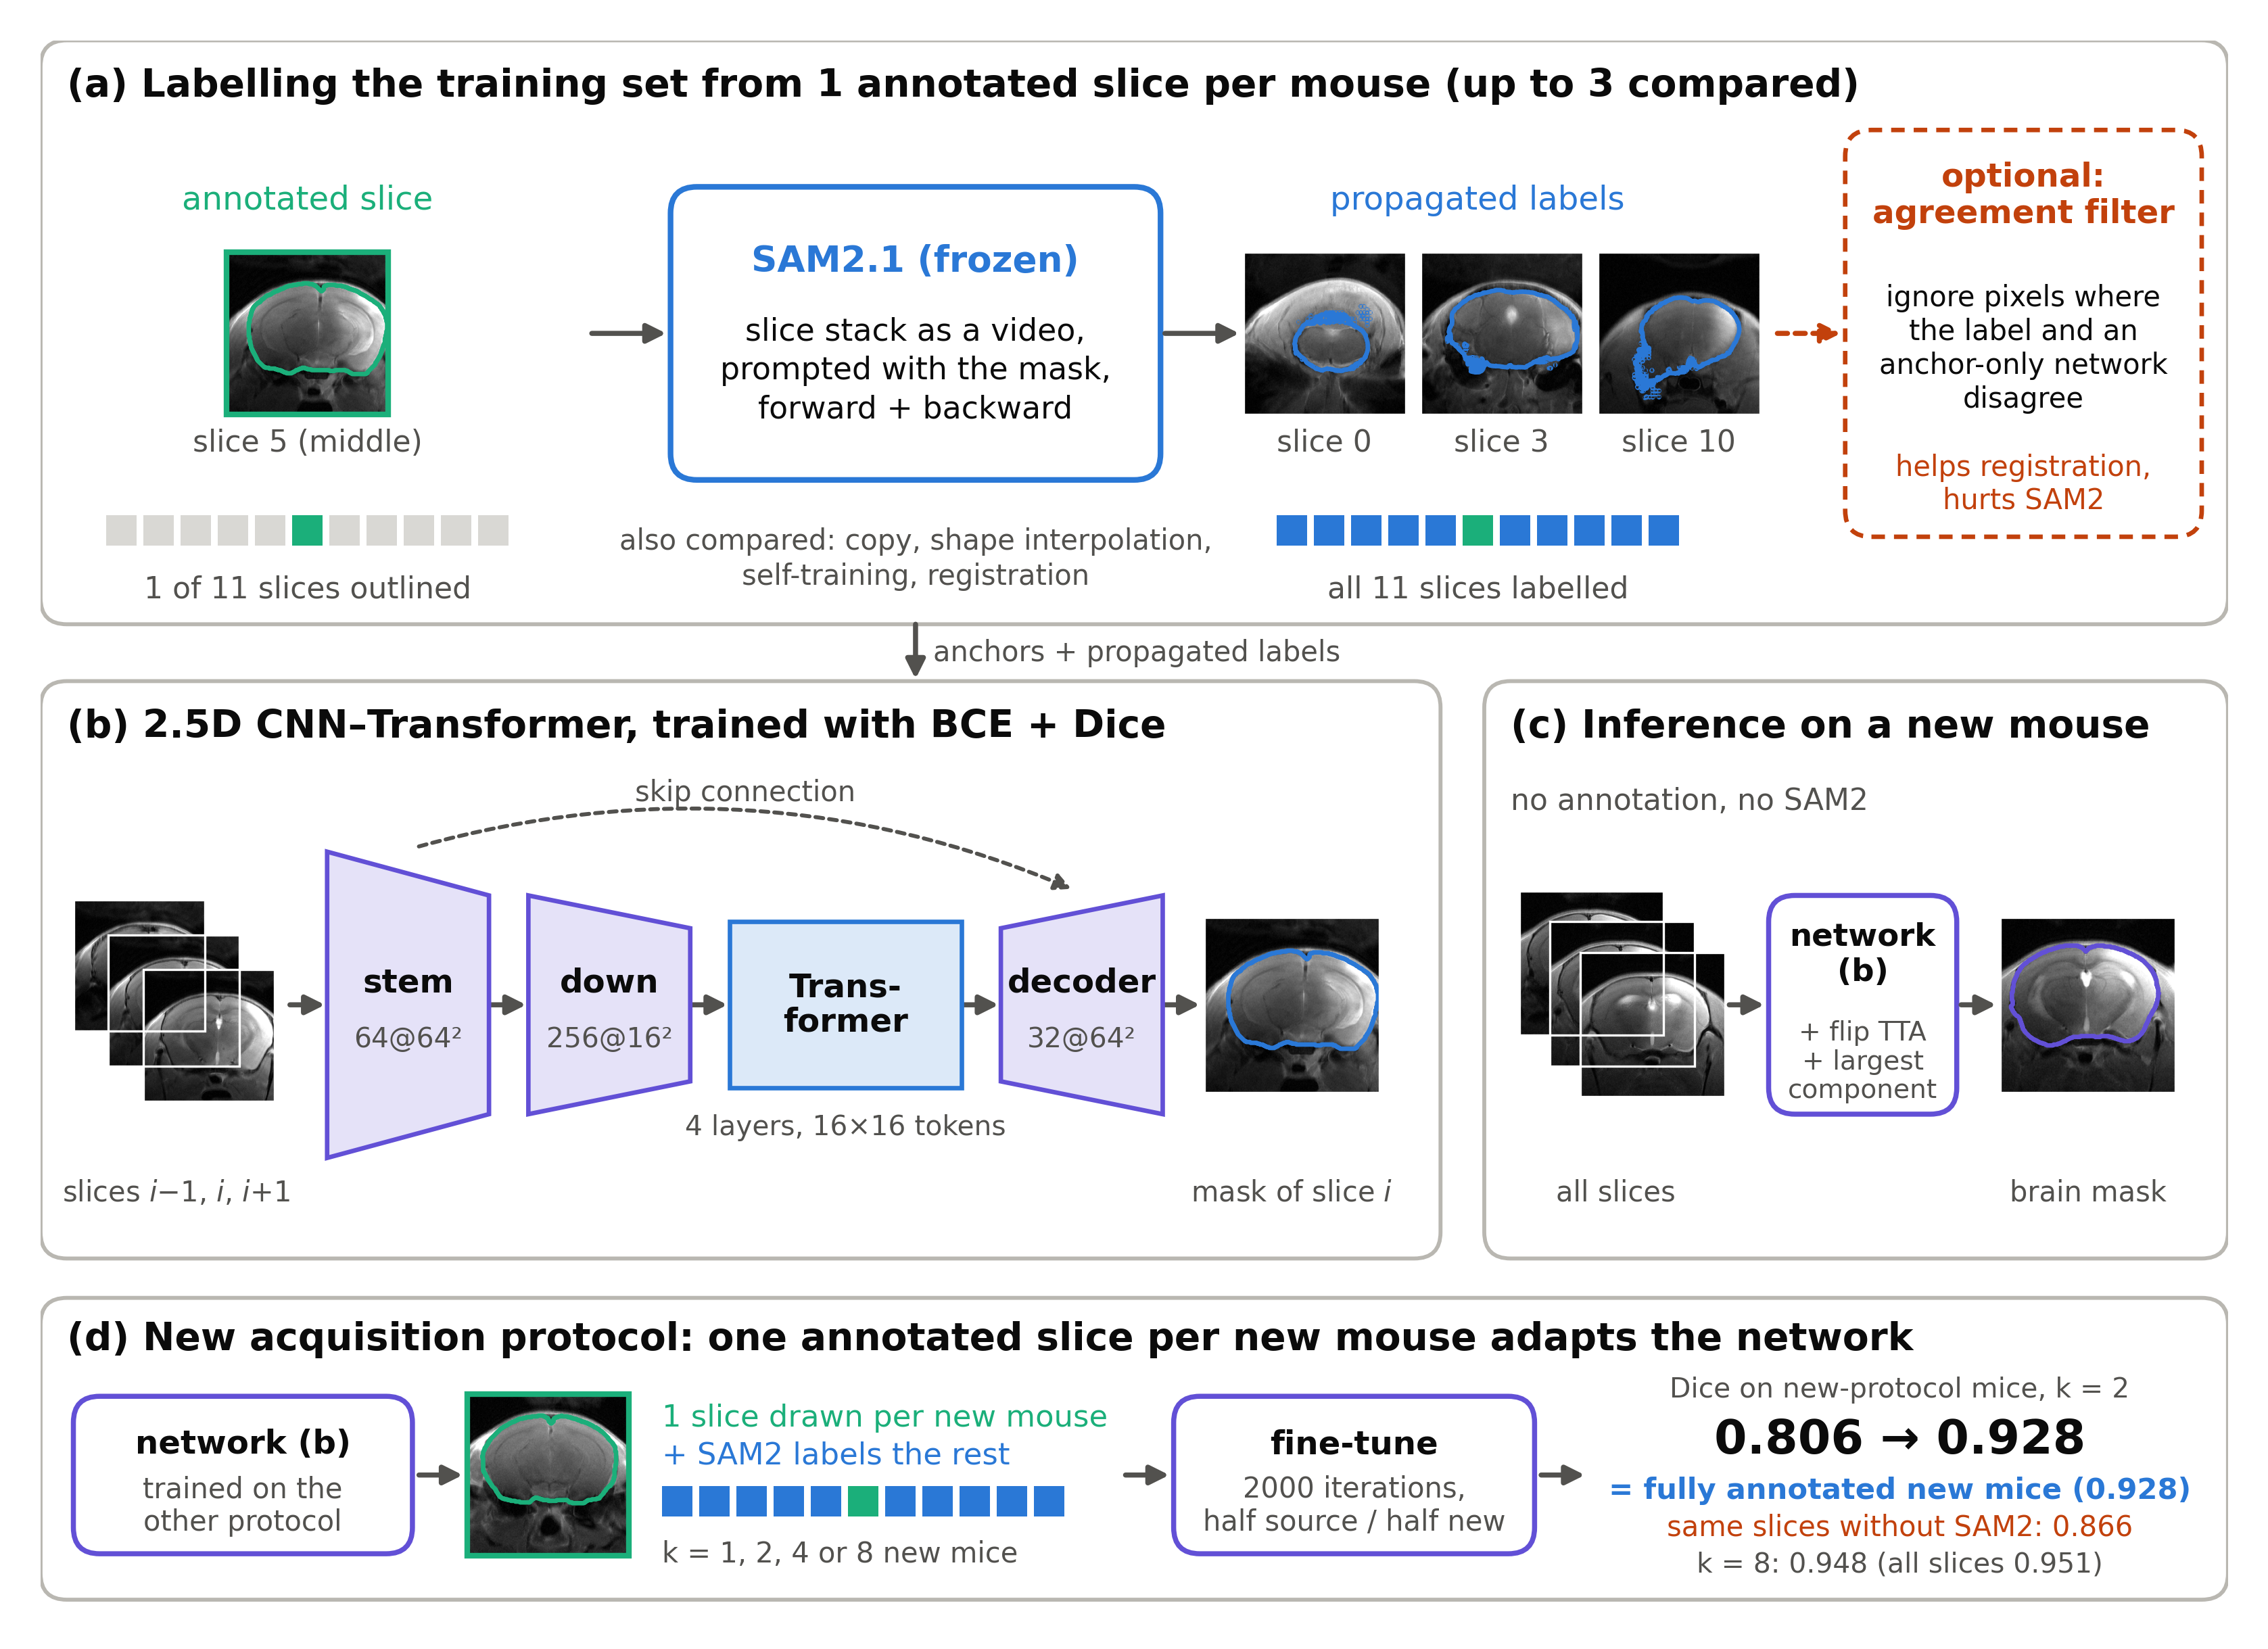
\includegraphics[width=0.70\linewidth]{fig_architecture_adapt.png}
\caption{Workflow. (a) One to three slices per training mouse are annotated (one shown), SAM2 propagates them to the other slices, and an optional filter ignores pixels where the label and an anchor-only network disagree. (b) The 2.5D CNN--Transformer predicts the centre-slice mask. (c) The trained network segments new mice without annotation or SAM2. (d) For a new protocol, the trained network is fine-tuned on one annotated slice per new mouse, with SAM2 labelling the rest (Sec.~\ref{sec:adapt}).}
\label{fig:overview}
\end{figure*}

\subsection{Data, annotation budget and network}

We used 20 mice from a 9.4~T Bruker scanner (axial T1/T2-weighted, 1~mm slices), each with 10 or 11 slices (218 in total) and expert brain masks, in two cohorts of ten with matrices of $256\times256$ and $200\times200$. Volumes were percentile-clipped (0.5, 99.5), scaled to $[0,1]$ and resampled to $256\times256$.

Only one to three slices of each training mouse, the anchors, were treated as annotated. Three anchors sat at $\lfloor n/4\rfloor$, $\lfloor n/2\rfloor$, $\lfloor 3n/4\rfloor$ (or at $1$, $\lfloor n/2\rfloor$, $n-2$, which bounds the ends of the stack; 28\% of slices), two at $\lfloor n/3\rfloor$, $\lfloor 2n/3\rfloor$ (18\%) and one at $\lfloor n/2\rfloor$ (9\%). Validation and test mice kept full masks for model selection and scoring only.

All methods trained the same 2.5D CNN--Transformer (Fig.~\ref{fig:overview}b; a slice and its two neighbours as input, a convolutional stem, a four-layer Transformer on $16\times16$ tokens and a decoder), for 8000 iterations with AdamW ($3\times10^{-4}$, cosine decay, batch 8), a weighted cross-entropy plus Dice loss and standard augmentation, keeping the best validation checkpoint. Inference added a flipped pass and kept the largest component.

\subsection{Propagators}
\label{sec:prop}

\textbf{SAM2.} Each volume was treated as a video and SAM2.1 (Hiera-L) \cite{ravi2024sam2}, without fine-tuning, was prompted with the anchor masks; forward and backward propagations were averaged.

\textbf{Registration.} A U-Net estimated displacement fields $\phi_{i\to i\pm1}$ between neighbouring slices at half resolution, trained with local normalised cross-correlation (window 9) and a smoothness penalty. An anchor-consistency loss requires the chained deformations to carry one anchor mask onto the next:
\begin{equation}
\mathcal{L}_{\text{anchor}} = 1 - \operatorname{Dice}\!\left(M_a \circ \phi_{a\to a\pm1} \circ \dots \circ \phi_{b\mp1\to b},\; M_b\right).
\end{equation}
Masks from the nearest anchors on both sides were averaged with inverse-distance weights. We also ran registration without $\mathcal{L}_{\text{anchor}}$.

\textbf{Baselines.} Copying the nearest anchor mask, shape-based interpolation of signed distance maps \cite{raya1990shape}, and self-training \cite{bai2017semi} on the predictions of an anchor-only network. Non-SAM2 propagators used three anchors.

\textbf{Pretraining and filtering.} As an alternative to propagation, the encoder was pretrained by masked image modelling \cite{ali2025ssl} on all training slices (4000 iterations) and fine-tuned on the anchors. For agreement filtering, a network trained on the anchors alone acted as a teacher, and pixels where it disagreed with the propagated label received zero loss weight. Registration kept the average of both maps; SAM2 kept its own label.

\subsection{Adaptation to a new protocol}
\label{sec:adapt}

We trained the network with full annotation on eight mice of one cohort (two more for checkpoint selection) and fine-tuned it on $k\in\{1,2,4,8\}$ mice of the other cohort, each with only its middle slice annotated. Target mice were split into five folds of two test mice, the first $k$ of the other eight being used, so each was tested once per $k$. Fine-tuning ran for 2000 iterations at $10^{-4}$, with half of each batch from source mice, and kept the final checkpoint. Target mice were supervised by the slice alone, with SAM2 labels, or with all slices annotated.

\subsection{Evaluation}

Cross-validation was five-fold at the animal level, stratified by cohort (14 training, two validation, four test mice per fold), with three seeds. Dice and slice-wise 95th-percentile Hausdorff distance (HD95, px) were averaged over seeds per mouse and compared with paired Wilcoxon tests. Non-inferiority used a one-sided paired Wilcoxon test with a 0.01 Dice margin, 2.4 times the seed-to-seed standard deviation (0.004). nnU-Net v2 \cite{isensee2021nnunet} (2D, 250 epochs, final checkpoint, same post-processing) was trained once per fold with full annotation, one slice plus SAM2 labels, or one slice with the rest ignored.

\section{Results}
\label{sec:results}

\begin{table}[t]
\centering
\caption{Test results on 20 mice, three anchors per training mouse. Label: Dice of propagated labels on unannotated slices. $^{*}$: different from anchors only ($p<0.05$). $^{\dagger}$: not different from full annotation.}
\label{tab:results}
\small
\setlength{\tabcolsep}{3pt}
\begin{tabular}{@{}lccc@{}}
\toprule
Method & Dice $\uparrow$ & HD95 $\downarrow$ & Label \\
\midrule
Anchors only & 0.924 & 13.2 & -- \\
+ copy nearest & 0.908$^{*}$ & 13.3 & 0.864 \\
+ shape interpolation & 0.909$^{*}$ & 12.8 & 0.871 \\
+ self-training & 0.927$^{*}$ & 12.6 & 0.893 \\
+ registration & 0.930 & 11.7 & 0.902 \\
+ reg., anchor loss & 0.931$^{*}$ & 11.2 & 0.906 \\
+ reg., anchor loss, agreement & 0.933$^{*}$ & 11.0 & 0.911 \\
+ SAM2 & \textbf{0.950}$^{*\dagger}$ & \textbf{8.9} & \textbf{0.940} \\
+ SAM2, agreement & 0.940$^{*}$ & 10.5 & 0.940 \\
\midrule
All slices annotated & 0.946 & 9.0 & -- \\
\bottomrule
\end{tabular}
\end{table}

\begin{table}[t]
\centering
\caption{Annotation budget: test Dice and HD95 (px) on 20 mice with one to three annotated slices per training mouse, alone or with SAM2 labels. Label: Dice of SAM2 labels. $^{\dagger}$: non-inferior to full annotation ($p<0.001$). n/a: not applicable. MIM: masked image pretraining, one slice (separate runs; own control 0.892 / 20.6).}
\label{tab:budget}
\small
\setlength{\tabcolsep}{3pt}
\begin{tabular}{@{}lcccccc@{}}
\toprule
 & & \multicolumn{2}{c}{Annotated only} & \multicolumn{3}{c}{+ SAM2} \\
\cmidrule(lr){3-4} \cmidrule(l){5-7}
Slices & \% & Dice & HD95 & Dice & HD95 & Label \\
\midrule
1 & 9 & 0.891 & 20.4 & \textbf{0.950}$^{\dagger}$ & 9.0 & 0.942 \\
2 & 18 & 0.925 & 13.4 & 0.949$^{\dagger}$ & 8.9 & 0.949 \\
3 & 28 & 0.924 & 13.2 & 0.950$^{\dagger}$ & 8.9 & 0.940 \\
All & 100 & 0.946 & 9.0 & n/a & n/a & n/a \\
\midrule
1 + MIM & 9 & 0.890 & 21.4 & n/a & n/a & n/a \\
\bottomrule
\end{tabular}
\end{table}

\begin{table}[t]
\centering
\caption{Adaptation: a network trained on one cohort is fine-tuned on $k$ mice of the other and tested on its held-out mice (10 mice, three seeds). Target labels: the middle slice of each mouse, plus SAM2 labels, or all slices. $^{\dagger}$: non-inferior to all slices at a 0.01 Dice margin ($p<0.05$).}
\label{tab:adapt}
\small
\setlength{\tabcolsep}{3pt}
\begin{tabular}{@{}clcccc@{}}
\toprule
 & & \multicolumn{2}{c}{$256\!\rightarrow\!200$} & \multicolumn{2}{c}{$200\!\rightarrow\!256$} \\
\cmidrule(lr){3-4} \cmidrule(l){5-6}
$k$ & Target labels & Dice & HD95 & Dice & HD95 \\
\midrule
0 & none & 0.932 & 11.3 & 0.806 & 33.1 \\
\midrule
1 & slice & 0.932 & 11.3 & 0.859 & 25.2 \\
 & + SAM2 & 0.937$^{\dagger}$ & 11.0 & 0.910$^{\dagger}$ & 17.8 \\
 & all & 0.930 & 10.5 & 0.910 & 17.6 \\
\midrule
2 & slice & 0.934 & 11.0 & 0.866 & 24.1 \\
 & + SAM2 & 0.941$^{\dagger}$ & 9.7 & 0.928$^{\dagger}$ & 14.6 \\
 & all & 0.941 & 9.1 & 0.928 & 14.6 \\
\midrule
4 & slice & 0.935 & 10.9 & 0.873 & 22.5 \\
 & + SAM2 & 0.943$^{\dagger}$ & 9.4 & 0.941$^{\dagger}$ & 11.8 \\
 & all & 0.940 & 9.1 & 0.944 & 11.3 \\
\midrule
8 & slice & 0.936 & 10.6 & 0.882 & 21.4 \\
 & + SAM2 & \textbf{0.945}$^{\dagger}$ & \textbf{8.8} & 0.948$^{\dagger}$ & 10.2 \\
 & all & 0.941 & 9.0 & \textbf{0.951} & \textbf{9.5} \\
\bottomrule
\end{tabular}
\end{table}

\begin{figure}[t]
\centering
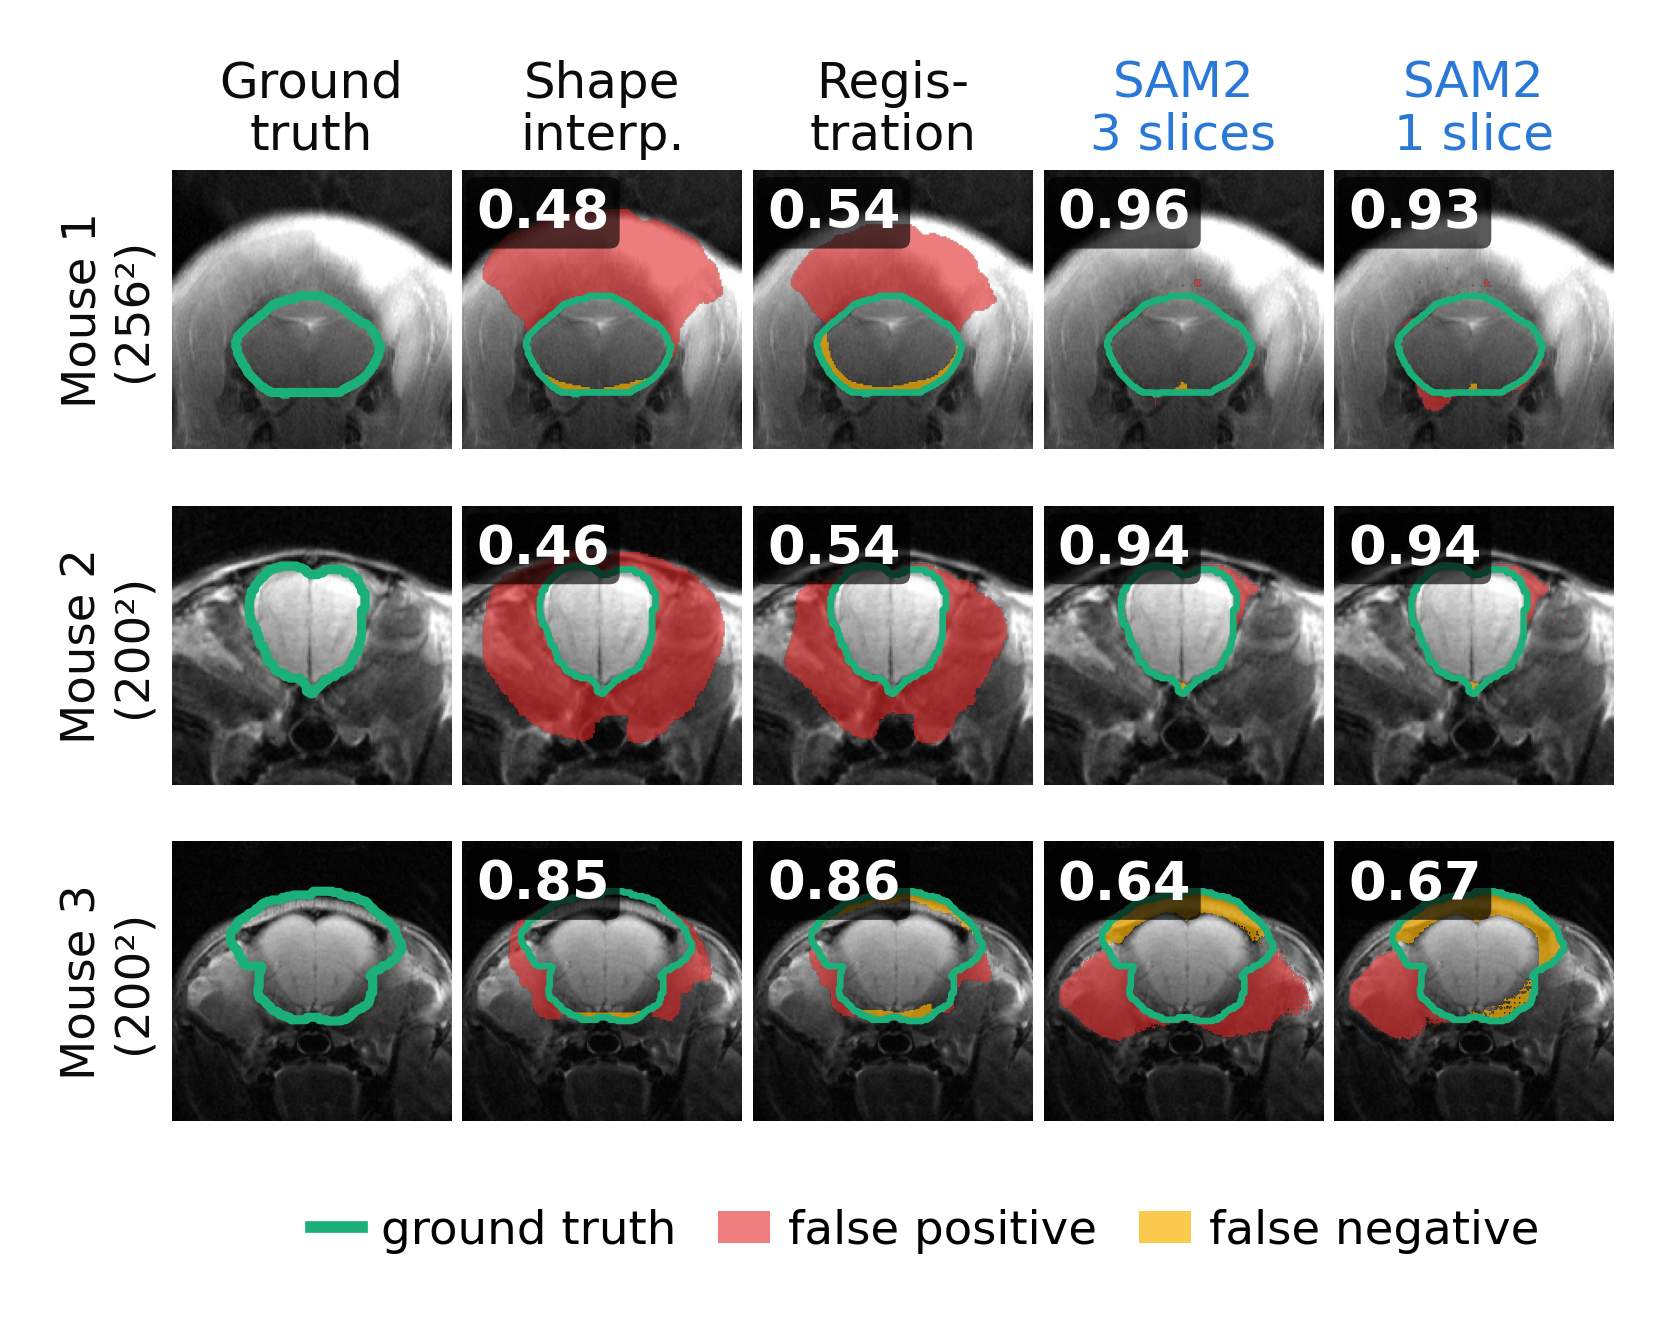
\includegraphics[width=0.70\linewidth]{fig_qualitative_pseudo_labels.png}
\caption{Propagated labels on an end slice, beyond the outermost anchor, of four training mice (two per cohort). Columns 2--5: three anchors; last column: SAM2 from the middle slice. Numbers: label Dice. Green: truth; red: false positive; amber: false negative; grey: excluded by filtering.}
\label{fig:qualitative}
\end{figure}

\textbf{One slice with SAM2 matches full annotation.} With three anchors (Table~\ref{tab:results}), the anchor-only network reached 0.924 against 0.946 with every slice annotated ($p<0.001$). SAM2 labels raised it to 0.950 and 8.9~px, better than anchors only and than the best registration variant on 19 of 20 mice each ($p<0.001$), and not different from full annotation in Dice ($p=0.96$) or HD95 ($p=0.76$), in both cohorts. With one annotated slice (Table~\ref{tab:budget}), training on it alone gave 0.891 and 20.4~px, while SAM2 labels gave 0.950 and 9.0~px, better on all 20 mice and non-inferior to full annotation ($p<0.001$). Masked image pretraining did not help (0.890 with one slice; 0.922 against 0.925 with three).

\textbf{Naive propagation hurts.} Copying and interpolation lowered Dice to 0.908 and 0.909, below anchors only. Their labels fell from 0.92--0.93 next to an anchor to 0.705 on the end slices beyond the last anchor (Fig.~\ref{fig:qualitative}), against 0.726 for self-training, 0.786 for registration and 0.883 for SAM2. Anchors at the stack ends helped the other propagators ($p<0.01$) but not SAM2.

\textbf{Filtering depends on the propagator.} Filtering ignored 2--3\% of unannotated pixels. It gave the best registration variant but reduced SAM2 to 0.940 ($p<0.001$): registration had labelled 57--60\% of the ignored pixels correctly, near chance, but SAM2 72--78\%, so filtering removed correct boundary supervision.

\textbf{nnU-Net.} With full annotation nnU-Net reached 0.960 and 6.9~px, 0.013 above our network. From one slice it fell to 0.868 alone but reached 0.958 and 7.6~px with SAM2 labels, non-inferior to full annotation ($p<0.001$).

\textbf{Two annotated slices adapt to a new protocol.} Trained on one cohort, the network lost little on the $200\times200$ cohort (0.932) but fell to 0.806 and 33.1~px on the $256\times256$ cohort, against 0.953 within it (Table~\ref{tab:adapt}). One annotated slice from one target mouse plus SAM2 already gave 0.910, equal to annotating that mouse fully and above the slice alone (0.859, $p=0.002$). With two mice, the slices alone gave 0.866 and with SAM2 labels 0.928, better on all ten test mice ($p=0.002$) and non-inferior to annotating both mice fully (0.928, $p=0.003$). Four and eight mice gave 0.941 and 0.948 against 0.944 and 0.951, both non-inferior; slices alone reached only 0.882 with eight. In the milder direction SAM2 labels beat the slices alone for $k\ge2$ (8 or 9 of 10 mice, $p\le0.010$; $k=1$: $p=0.064$) and were non-inferior to full annotation.

\section{Discussion and conclusion}
\label{sec:discussion}
One annotated slice per mouse and a promptable video model replaced slice-by-slice annotation for training a brain extraction network, with 91\% fewer annotated slices and no loss beyond a 0.01 Dice margin. The same recipe made a new protocol cheap: two annotated slices restored a network from 0.806 to 0.928, as well as full annotation. A propagator that cannot follow anatomy beyond the annotated slices is worse than none, and agreement filtering helps only a propagator near chance where it acts.

Limits: 20 mice from one scanner, whole-brain masks only, and annotation time was not measured. Cross-validation used two fully annotated validation mice per fold. Adaptation was tested between two protocols of one scanner and should be confirmed across sites.

\section{Compliance with ethical standards}
\label{sec:ethics}
\todo{Animal study approval: institution and protocol number (IACUC) for the MRI data, from coauthors.}

\section{Acknowledgments}
\label{sec:acknowledgments}
\todo{Funding sources; or state that no funding was received.} The authors have no relevant financial or non-financial interests to disclose.

% References (formatted IEEEbib style; no refs.bib or BibTeX needed)
{\small
\begin{thebibliography}{10}

\bibitem{hsu2020skullstripping}
Li-Ming Hsu, Shuai Wang, Paridhi Ranadive, et~al.,
\newblock ``Automatic skull stripping of rat and mouse brain {MRI} data using
  {U-Net},''
\newblock {\em Frontiers in Neuroscience}, vol. 14, pp. 568614, 2020.

\bibitem{defeo2021munet}
Riccardo De~Feo, Artem Shatillo, Alejandra Sierra, et~al.,
\newblock ``Automated joint skull-stripping and segmentation with {Multi-Task
  U-Net} in large mouse brain {MRI} databases,''
\newblock {\em NeuroImage}, vol. 229, pp. 117734, 2021.

\bibitem{ali2025ssl}
Tayyab Ali, Xin Huang, Miroslaw Janowski, et~al.,
\newblock ``A self-supervised framework for automated mouse brain extraction in
  data-constrained {MRI} studies,'' 2025,
\newblock TODO: venue, year and pages of the previous paper.

\bibitem{cicek2016unet3d}
{\"O}zg{\"u}n {\c{C}}i{\c{c}}ek, Ahmed Abdulkadir, Soeren~S. Lienkamp, et~al.,
\newblock ``{3D U-Net}: Learning dense volumetric segmentation from sparse
  annotation,''
\newblock in {\em Medical Image Computing and Computer-Assisted Intervention
  (MICCAI)}, 2016, pp. 424--432.

\bibitem{raya1990shape}
Sai~Prasad Raya and Jayaram~K. Udupa,
\newblock ``Shape-based interpolation of multidimensional objects,''
\newblock {\em IEEE Transactions on Medical Imaging}, vol. 9, no. 1, pp.
  32--42, 1990.

\bibitem{balakrishnan2019voxelmorph}
Guha Balakrishnan, Amy Zhao, Mert~R. Sabuncu, et~al.,
\newblock ``{VoxelMorph}: A learning framework for deformable medical image
  registration,''
\newblock {\em IEEE Transactions on Medical Imaging}, vol. 38, no. 8, pp.
  1788--1800, 2019.

\bibitem{ravi2024sam2}
Nikhila Ravi, Valentin Gabeur, Yuan-Ting Hu, et~al.,
\newblock ``{SAM 2}: Segment anything in images and videos,''
\newblock in {\em International Conference on Learning Representations (ICLR)},
  2025.

\bibitem{ma2024medsam}
Jun Ma, Yuting He, Feifei Li, et~al.,
\newblock ``Segment anything in medical images,''
\newblock {\em Nature Communications}, vol. 15, pp. 654, 2024.

\bibitem{zhu2024medicalsam2}
Jiayuan Zhu, Abdullah Hamdi, Yunli Qi, et~al.,
\newblock ``Medical {SAM} 2: Segment medical images as video via segment
  anything model 2,'' 2024,
\newblock arXiv:2408.00874.

\bibitem{chen2025slmsam2}
Yuwen Chen, Zafer Yildiz, Qihang Li, et~al.,
\newblock ``Accelerating volumetric medical image annotation via short-long
  memory {SAM} 2,'' 2025,
\newblock arXiv:2505.01854.

\bibitem{zhang2025nnsam2}
Zhongyi Zhang, Julie~A. Hides, Enrico De~Martino, et~al.,
\newblock ``{nnSAM2}: {nnUNet}-enhanced one-prompt {SAM2} for few-shot
  multi-modality segmentation and composition analysis of lumbar paraspinal
  muscles,'' 2025,
\newblock arXiv:2510.05555.

\bibitem{yu2022ben}
Ziqi Yu, Xiaoyang Han, Wenjing Xu, et~al.,
\newblock ``A generalizable brain extraction net ({BEN}) for multimodal {MRI}
  data from rodents, nonhuman primates, and humans,''
\newblock {\em eLife}, vol. 11, pp. e81217, 2022.

\bibitem{bai2017semi}
Wenjia Bai, Ozan Oktay, Matthew Sinclair, et~al.,
\newblock ``Semi-supervised learning for network-based cardiac {MR} image
  segmentation,''
\newblock in {\em Medical Image Computing and Computer-Assisted Intervention
  (MICCAI)}, 2017, pp. 253--260.

\bibitem{isensee2021nnunet}
Fabian Isensee, Paul~F. Jaeger, Simon A.~A. Kohl, et~al.,
\newblock ``{nnU-Net}: a self-configuring method for deep learning-based
  biomedical image segmentation,''
\newblock {\em Nature Methods}, vol. 18, no. 2, pp. 203--211, 2021.

\end{thebibliography}
}

\end{document}